\chapter{Polyline Simplification}
\label{chap:simplify_polyline}
\ccChapterAuthor{Ovidiu Grigore and Remco Veltkamp}


\section{Introduction}

This package offers several algorithms for the simplification of a
polyline. Input and output are a sequence of points.  The user can
specify either the desired number of points of the simplified polyline,
or the maximal acceptable error. This package offers optimal methods, like
dynamic programming \cite{[cgal:gt-dpasrcp-93]}, and sub-optimal methods, 
like recursive split \cite{[dp-arnpr-73]}. The optimal methods
are slower and need more memory.

All these algorithms are implemented in a generic manner. Depending on
the application, the user can choose features like: the coordinate type of the
points (\ccc{int}, \ccc{double}, \ccc{leda_integer}, \ccc{Gmpz},
etc.), the kernel representation (\ccc{Cartesian}, \ccc{Homogeneous}),
as well as the distance used in measuring the approximation error.
Different kinds of distances between a point and a segment are available. 
There are common distances like: the Euclidean distance, the Manhattan distance,
the $L_\infty$ distance, measured to the supporting line or to the segment, but
also other distances, like the bounding shell distance \cite{[cgal:v-hal-94]}. 

In the same spirit of generalization, the approximation error can be assessed either as
the maximum value of all the distances computed between the input
polyline and the simplified polyline, or as the sum of all
these distances.

Although the interface is generic, this package implements faster algorithms
for the the Euclidean distance, namely the incremental algorithm \cite{[cgal:pv-opadc-94]},
and the algorithm based on the path hull structure \cite{[hs-sudpl-92]}.

Finally, another group of algorithms, optimal polyline simplification methods
for particular distance measures, are offered. They are generic
as far as the coordinate type of the points and the kernel type are
concerned, but these methods use graph search techniques \cite{[cgal:ii-pac]} to
perform the polyline simplification and only work with the Euclidean distance error
assessment.

\section{Definitions}

Let $\{p_1, \ldots, p_N\}$ be a sequence of successive points, defining the
input polyline, then, with respect to a given criterion, it can be
simplified to a sequence with a reduced number of points $\{q_1,\ldots, q_M\}$, $M<N$.

\begin{figure}[h]
\begin{ccTexOnly}
\begin{center}
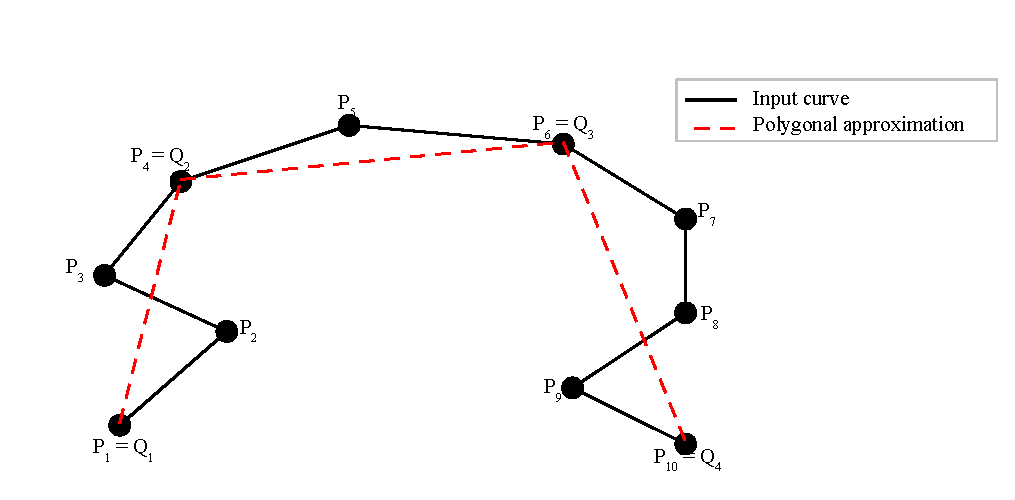
\includegraphics[width=10cm]{Polygonal_approximation_d/fig1} 
\end{center}
\end{ccTexOnly}
\caption{Polyline simplification.
\label{Simplification_Fig_intor}}
\begin{ccHtmlOnly}
<CENTER>
<img border=0 src="./tr1.gif" width=300>
</CENTER>
\end{ccHtmlOnly}
\end{figure} 

To define the differences (roughness) between the input and the output
polyline, two parameters can be used: the
decrease in the number of points  ($N-M$)
and the error of approximation that measures the changing of the input
polyline.  

Depending on the main parameter of interest, there are two possible
approaches that can to be used for solving a polyline simplification
problem: 

\begin{description} 

\item[min-$\#$:] when given an upper bound on the error, compute the simplified polyline
with the minimum number of points.

\begin{figure}[h]
\begin{ccTexOnly}
\begin{center}
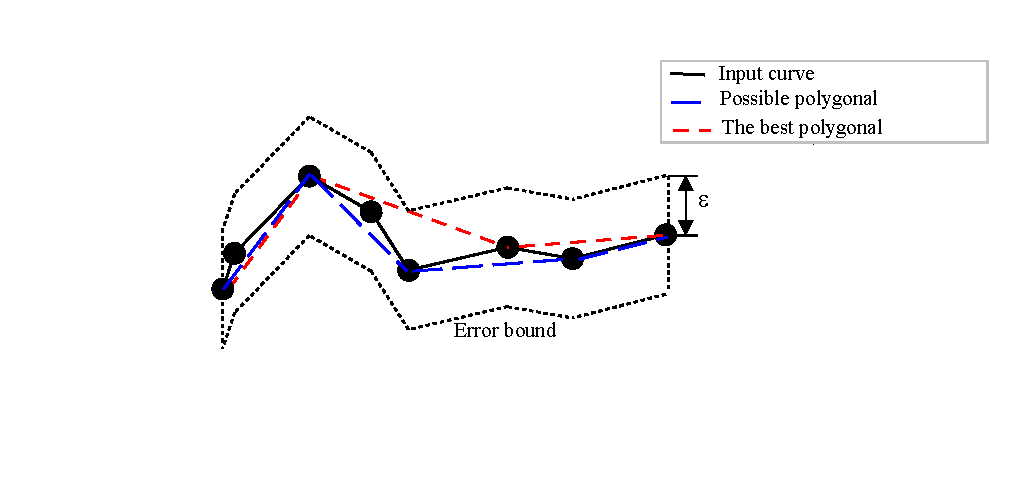
\includegraphics[width=10cm]{Polygonal_approximation_d/fig2} 
\end{center}
\end{ccTexOnly}
\caption{Min-$\#$ polyline simplification approach.
                    For a given error threshold $\epsilon$, the polyline 
                 that has minimum number of point is chosen.
\label{Simplification_Fig_min_nr}}
\begin{ccHtmlOnly}
<CENTER>
<img border=0 src="./fig1.gif" width=300>
</CENTER>
\end{ccHtmlOnly}
\end{figure}



\item[min-$\epsilon$:] when given the desired number of points of 
the simplified polyline, compute the polyline that approximates as
good as possible the input polyline for a given error function
(Figure~\ref{Simplification_Fig_min_eps}).

\begin{figure}[h]
\begin{ccTexOnly}
\begin{center}
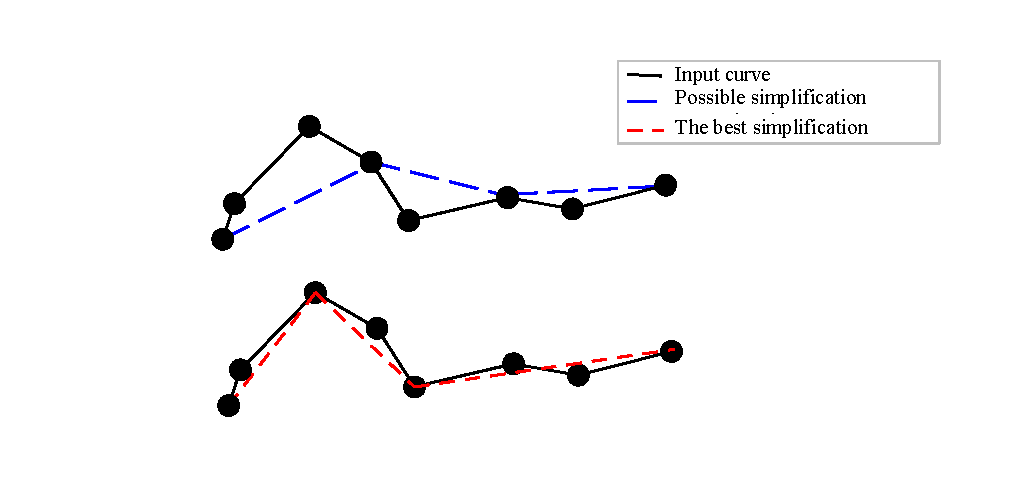
\includegraphics[width=10cm]{Polygonal_approximation_d/fig3} 
\end{center}
\end{ccTexOnly}
\caption{Min-$\epsilon$ polyline simplification approach.
              Given an $M=4$, several approximations could be done. 
                           The output one minimizes the approximation error.
\label{Simplification_Fig_min_eps}}
\begin{ccHtmlOnly}
<CENTER>
<img border=0 src="./fig3.gif" width=300>
</CENTER>
\end{ccHtmlOnly}
\end{figure}



\end{description}


\section{Approximation Error Assessments}

For both categories of algorithms an evaluation of the error
of the simplified polyline is needed. To estimate it,
several distances from a point to a line can be applied, such as: the
Euclidean distance, the Manhattan distance, the $L_\infty$ distance, the
vertical distance, the bounding shell distance.

Also, the error obtained when approximating a polyline fragment with a
line segment can be defined either as the maximum value of the
distances between the segment and each point of the polyline portion or
as the sum of these distances.

One main group of distances consists of particular cases of the
general distance $L_p$. For two points $v$ and $w$ from a $k$-dimensional space
it is defined as:

$$ L_p(v,w) = (\sum_{i=1}^k{| v_i - w_i|^p})^{1/p} $$

where $v_i$ and $w_i$ are the $i$-th coordinate of the $v$ and $w$, respectively.  

\subsection{Euclidean Distance}

Maybe the mostly used distance is the Euclidean one, obtained from the general formula for $p=2$:

$$L_2 (v, w) = \sqrt{(v_x - w_x)^2 + (v_y - w_y)^2}
 
In Figure~\ref{Simplification_Fig_Euclidean} the distance between a point and a line is shown. 


\begin{figure}[h]
\begin{ccTexOnly}
\begin{center}
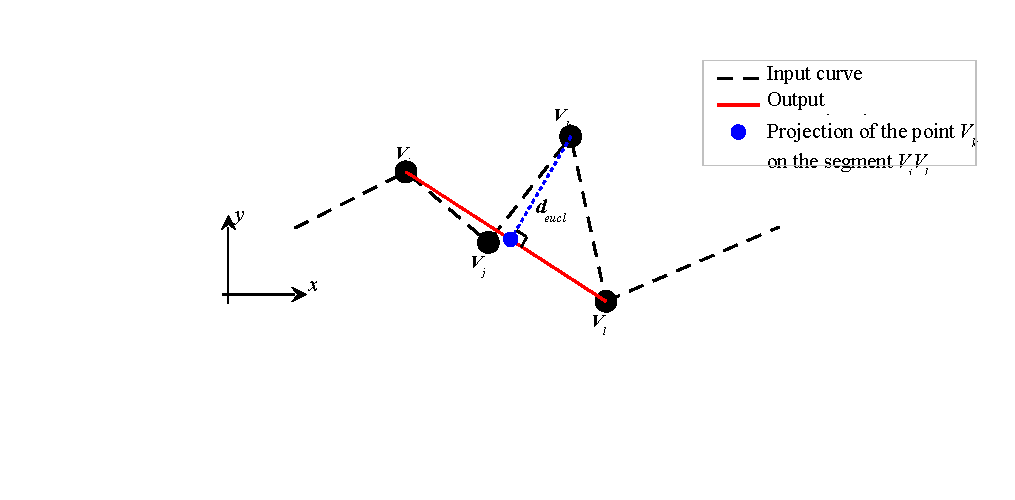
\includegraphics[width=10cm]{Polygonal_approximation_d/fig5} 
\end{center}
\end{ccTexOnly}
\caption{Euclidean distance measurement (deucl).
\label{Simplification_Fig_Euclidean}}
\begin{ccHtmlOnly}
<CENTER>
<img border=0 src="./fig5.gif" width=300>
</CENTER>
\end{ccHtmlOnly}
\end{figure}



\subsection{Manhattan Distance}

For $p=1$ the distance obtained is usually called Manhattan distance or
city block distance. For a $(x,y)$ plane, it is defined as:

$$L_1 (v, w) = | v_x - w_x | + | v_y - w_y | $$

This distance is equal to the length of the shortest path between the
two points while going only along the axis directions. In Figure~\ref{Simplification_Fig_Manhattan} is
presented the measure of the Manhattan distance between a point and a
segment.

\begin{figure}[h]
\begin{ccTexOnly}
\begin{center}
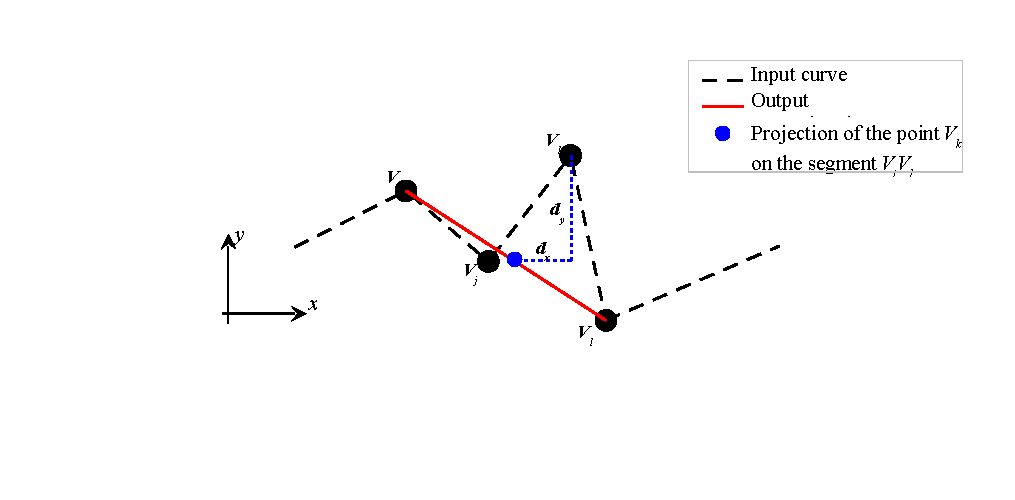
\includegraphics[width=10cm]{Polygonal_approximation_d/fig4} 
\end{center}
\end{ccTexOnly}
\caption{Manhattan distance measurement $(d_x+d_y)$.
\label{Simplification_Fig_Manhattan}}
\begin{ccHtmlOnly}
<CENTER>
<img border=0 src="./fig4.gif" width=300>
</CENTER>
\end{ccHtmlOnly}
\end{figure}





\subsection{Max Distance}

$L_\infty$ is the particular case obtained for $ p \rightarrow \infty$, when, for a $k$-dimensional space, the formula becomes:

$$ L_\infty (v, w) = \max_{i=1,\ldots,k}{ | v_i - w_i | } $$

where $v_i$ and $w_i$ are the $i$-th coordinate of the points $v$ and $w$, respectively.  
As is easy to observe, to measure the $L_\infty$ distance is similar to the $L_1$ procedure (Fig. 4), 
but this time only the maximum value of the distances computed along the axis is taken into account. 

\subsection{Vertical Distance}

The vertical distance is equal to the difference in $y$-values between
the current point and the intersection point of the vertical line that
is passing through it and the supporting line of the approximation
segment. Figure~\ref{Simplification_Fig_Vertical}.a illustrates the case
when the intersection point is inside the segment and Figure~\ref{Simplification_Fig_Vertical}.b. 
illustrates the case when the intersection point is outside the segment.


\begin{figure}[h]
\begin{ccTexOnly}
\begin{center}
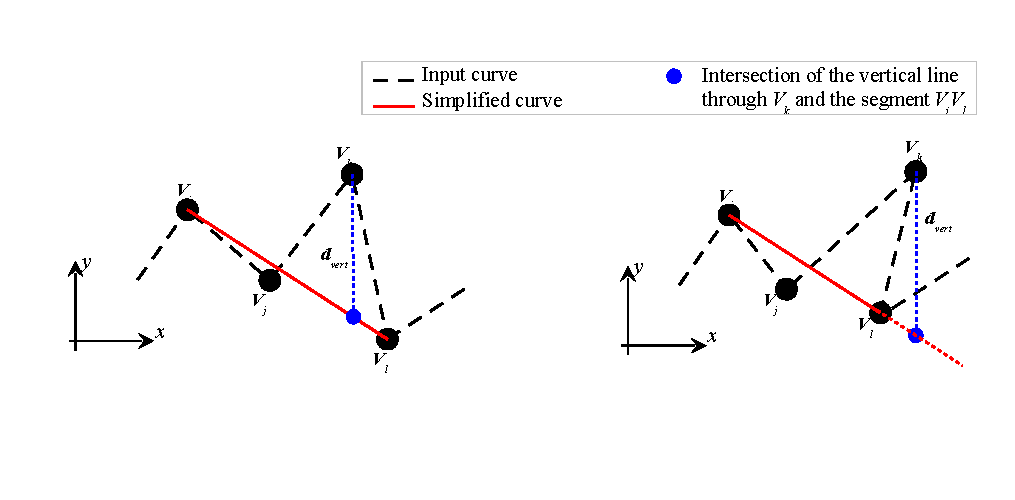
\includegraphics[width=15cm]{Polygonal_approximation_d/fig6} 
\end{center}
\end{ccTexOnly}
\caption{Vertical distance measurement.
\label{Simplification_Fig_Vertical}}
\begin{ccHtmlOnly}
<CENTER>
<img border=0 src="./fig6.gif" width=300>
</CENTER>
\end{ccHtmlOnly}
\end{figure}


Note that when this distance is used to assess polylines that contain
vertical parts, these cannot be practically approximated. In that case
the vertical parts are returned unchanged.


\subsection{ Bounding Shell Distance }

The shell is a bounding volume for the polyline segment that has to be
simplified. It consists of the two smallest circle arcs passing
through the two end points of the approximating segment that includes
between them all the points of the polyline portion to be
approximated. If all the points are on the same side of the
approximating segment then the bound on the side without points is the
segment itself. The distance associated to a bounding shell is defined
as the maximum value of the Euclidean distances measured between the
segment and all the points of the two bounding arcs \cite{[cgal:v-hal-94]}.

\begin{figure}[h]
\begin{ccTexOnly}
\begin{center}
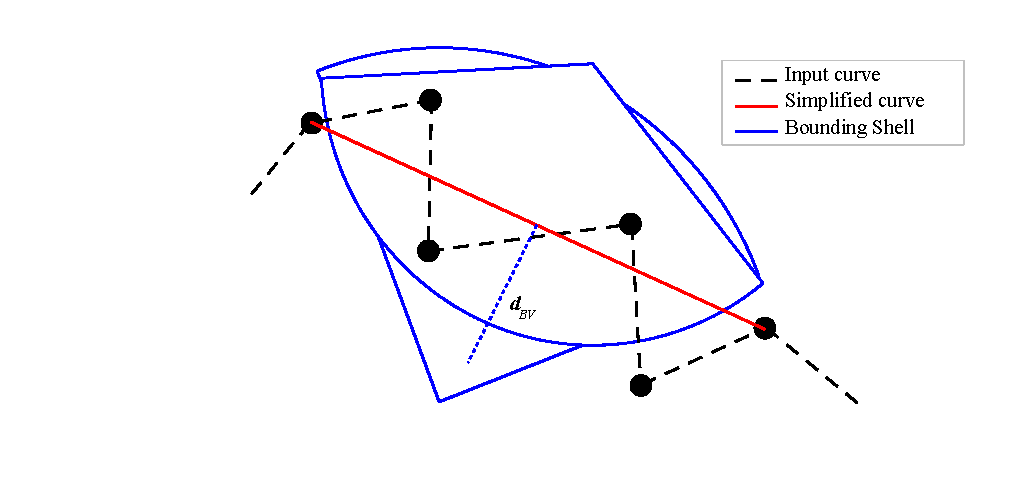
\includegraphics[width=10cm]{Polygonal_approximation_d/fig7} 
\end{center}
\end{ccTexOnly}
\caption{Finding the bounding volume and its associated distance.
\label{Simplification_Fig_Bounded}}
\begin{ccHtmlOnly}
<CENTER>
<img border=0 src="./fig7.gif" width=300>
</CENTER>
\end{ccHtmlOnly}
\end{figure}




\subsection{Distance Measured to the Segment or to the Supporting Line}

Whenever the procedure of measuring the distance between a point and a
segment implies the projection of the point on the segment, there are
two possible cases: either the projection point is inside the segment
or it is outside. Therefore, two kinds of distances can be assessed:

\begin{itemize}
\item the distance measured to the supporting line of the segment; in this
case the distance is computed always between the point and its
projection, even if it is outside of the segment, on its supporting line.

\item the distance measured to the segment; this time two cases can
happen: first, when the projection of the point is inside the segment
and the distance is computed similarly with case (a); in the second
approach the projection is on the supporting line, outside the segment,
so it is chosen the closest point from the segment, actually the
closest end point of the segment, to the current point.
\end{itemize}






\begin{figure}[h]
\begin{ccTexOnly}
\begin{center}
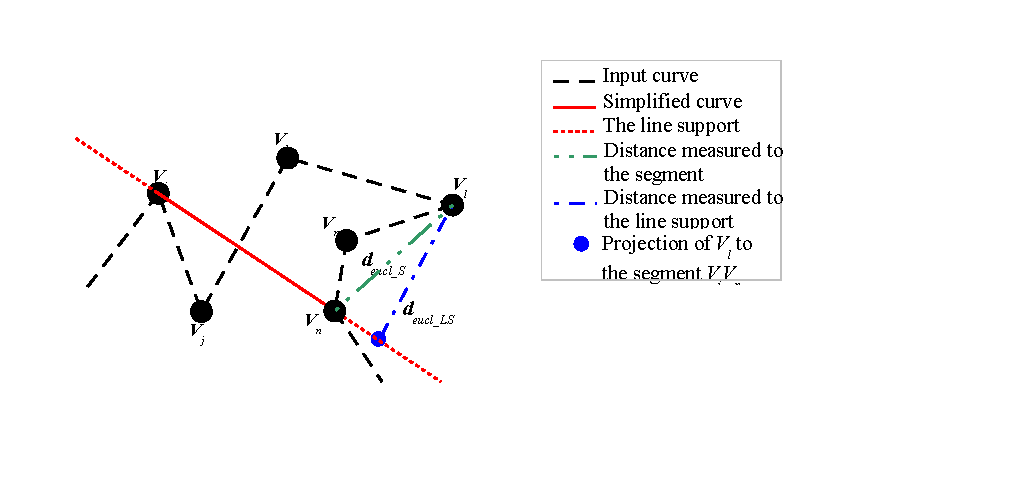
\includegraphics[width=12cm]{Polygonal_approximation_d/fig8} 
\end{center}
\end{ccTexOnly}
\caption{Measuring distance to the supporting line or to the segment.
          The difference between the two approaches is presented 
           for the Euclidean distance.
\label{Simplification_Fig_LineSegment}}
\begin{ccHtmlOnly}
<CENTER>
<img border=0 src="./fig8.gif" width=300>
</CENTER>
\end{ccHtmlOnly}
\end{figure}




\section{Polyline Simplification Algorithms}	

\subsection{Optimal and Sub-Optimal Solutions}


Two parameters characterize the polyline simplification of an input
polyline: its number of vertices $M$ and the error $\epsilon$ of
the simplified polyline. Setting an upper bound for one of these
parameters, the value of the other one depends on the algorithm that
is applied, but the smaller the value the better the algorithm. So,
from this point of view, the polyline simplification methods can be
split in two main groups: the bounded-error algorithms, when the upper
bound of the approximation error is given, and the
bounded-number-of-points algorithms, when the upper bound for the
number of vertices of the output polyline is given.

According to the accuracy of their solution, we can roughly divide the
algorithms used to approximate polylines into two main
categories: the optimal and the sub-optimal methods.

In the former case, optimization techniques, like dynamic programming,
are applied to find the best solution of the approximation
problem. Therefore, in this case, the bounded-$\#$ problem is equivalent
with a min-$\epsilon$ approach (Section 1.2, page 4) and the bounded-$\epsilon$ with the
min-$\#$ (Section 1.2, page 5).

Generally, these algorithms have relative slow running time, even
though there existed attempts to implement faster optimal algorithms
for some specific error measurements, such as the incremental
technique made by Perez and Vidal \cite{cgal:pv-opadc-94} for the Euclidean and vertical
distances measured to the supporting line of the segments.

The latter group of algorithms tried to be a compromise between the
loss of precision of the solution and the improvement of their running
time. Usually, they are based on heuristic techniques, such as the
recursive split method, that offers a faster running time, but the
solution is not as good as for the optimal one.

To understand the difference in running time of the several kinds of
algorithms, in Table 1 are presented the time complexity limits for
some of them. $n$ denotes the number of points of the input polyline and $m$
represents the number of points of the output approximation. The usual
implementation cases, which do not use special data structures or
techniques, are named in table by {\em general implementation}.


\begin{tabularx}{10cm}{|L|L}
Algorithm and implementation specification &  Time complexity of computing \\ 
Recursive Split, \cite{dp-arnpr-73}
General implementation                     &  $O(N^2)$ \\
Recursive Split, 
Maximum Squared Euclidean Distances, Path Hull implementation [1]
                                           & $O(N \log N)$ \\
Dynamic Programming, \cite{cgal:gt-dpasrcp-93}
General implementation
                                           & $O(MN^3)$ \\
Dynamic Programming, new implementation
General implementation                     & $O(N^3)$\\

Dynamic Programming 
Sum of Euclidean Distances, Incremental technique \cite{cgal:pv-opadc-94}
                                           & $O(MN^2)$ \\
Graph Search Method, \cite{cgal:ii-pac}
Maximum of Euclidean Distances, measured to supporting line
                                           & $O(N2\log N)$ \\
Graph Search Method, 
Sum of Euclidean Distances, measured to supporting line
                                           & $O(N^3)$\\
\end{tabularx}


\subsection{Dynamic Programming Method}

Dynamic programming is a technique used in solving optimization
problems, this time applied to finding the optimal simplification
for a given polyline and the desired
parameters. Generally speaking, its main idea is to build the final
optimum by finding optimum solution at the partial problems. It finds
first the optimum solution of the simplest possible level of the
problem. Each time the next level is more complex than the previous
one, but computing the optimum solution of the current level is based
on the optimum solutions found in all bottom levels. In the final
level, when the partial problem overlapped the initial problem, the
global optimal solution is found.

In the case of polyline simplification problems, the dynamic
programming technique starts with computing all the simplifications of
all possible parts of the input polyline using only one segment:

$${ \Delta( 1, n ) }_{n=1\ldots N} $$

After this, step by step, the simplifications of the polyline using an increasing number of segments ${2, 3, \ldots,M}$ 
are computed using an iterative process based of the following formula:

$$ \Delta(n,m) = \left\{ \begin{array}{l,l}
\Delta(1,n), & n \geq m = 2\\
\mathop{\min}_{m-1 \leq i \leq n-1}{\Delta(i,m-1)+\Delta(i,n)}, & n \geq m > 2 \end{array}  \right.  $$ 


\subsection{Recursive Split Method}

This algorithm is a heuristic approach, finding a sub-optimal, but
often good, solution of the simplification problem, the main aim being
the improvement of the other features of the optimal algorithms, like
running time and the memory usage.

Actually, the recursive split method is based on a {\em divide and
conquer} technique. It starts with the initial segment that links
the two end points of the input polyline, for which the furthest point is
found. If the distance from the furthest point to the segment is
greater than a given error threshold, then the problem is split into
two similar sub-problems: approximating the two polyline portions, one
from the start point to the furthest point, the second from the
furthest point to the end point. So, the algorithm is repetitively
applied until all the segments obtained approximate their polyline
portion with an error less then the given threshold.


\begin{figure}[h]
\begin{ccTexOnly}
\begin{center}
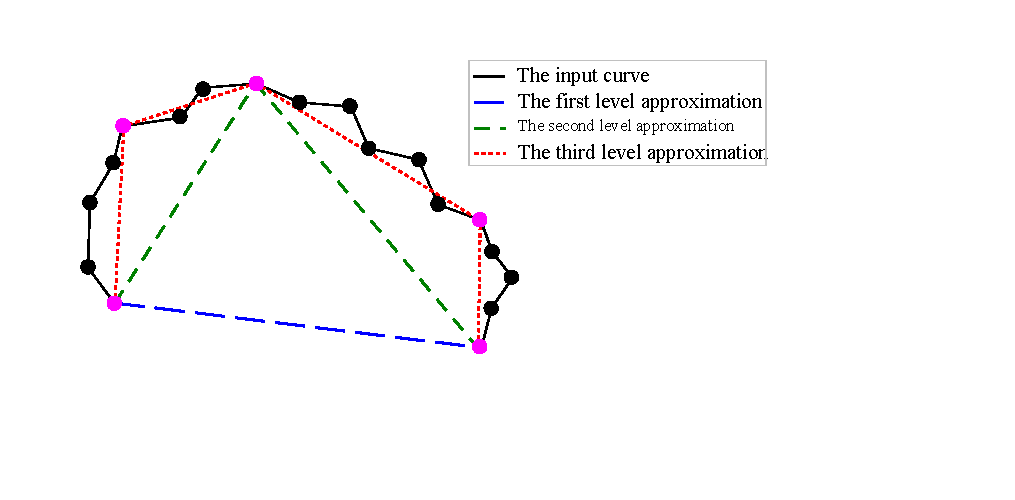
\includegraphics[width=10cm]{Polygonal_approximation_d/fig8-2} 
\end{center}
\end{ccTexOnly}
\caption{Example of  applying the recursive split method.
\label{Simplification_Fig_RecursiveSplit}}
\begin{ccHtmlOnly}
<CENTER>
<img border=0 src="./fig8-2.gif" width=300>
</CENTER>
\end{ccHtmlOnly}
\end{figure}




\section{Example}

In the following example we read a polyline from the console and generate
a simplified polyline with half the number of vertices. We use the recursive
split method which is also called the {\em Douglas-Peucker algorithm}.

\ccIncludeExampleCode{../examples/Polygonal_approximation_d/douglas-peucker.C}



